\clearpage
\begin{column}{コロナ前後における活動の変化}
\subsubsection{MDCEVモデルとRecursive Logit Modelの比較}

構造型モデルである\textbf{MDCEVモデル}と\textbf{Recursive Logit Model}の比較を行った．
\textbf{MDCEVモデル}は，1日を観測単位として，活動への時間配分を「離散的な活動選択＋連続的な時間配分」として定式化するものである．
一方で，離散選択モデルである\textbf{Recursive Logit Model}は1日を時間ステップ列とみなし，1ステップ列からの遷移列から学習するものである．
場所次元と過去活動の効果は両方とも無視するものとし，「時間配分」と「時系列推移」の2つのモデルでそれぞれ何を表現するか，できるかを比較する．
東京都市圏で実施された4つのPPデータを使用するものとする．

\begin{center}
  \renewcommand{\arraystretch}{1.5}
  \setlength{\tabcolsep}{14pt}

  \begin{tabular}{cllr}
    \toprule
    \textbf{period} & \textbf{期間} & \textbf{文脈} & \textbf{n\_users (raw)} \\
    \midrule
    1 & 2019-07-08 .. 2020-02-11 & \textbf{コロナ前} & 305 \\
    2 & 2021-10-03 .. 2021-11-25 & \textbf{コロナ規制明け直後} & 115 \\
    3 & 2022-12-19 .. 2023-01-30 & コロナ後・冬 & 182 \\
    4 & 2023-11-15 .. 2023-11-29 & コロナ後・秋 & 223 \\
    \bottomrule
  \end{tabular}
  \captionof{table}{東京都圏で実施された4つのPP調査}
  \label{tab:pp-survey-tokyo}
\end{center}

活動カテゴリとしては，H(home)，S(Shopping)，W(Commute/Work)，W2(Business)，O(Other)，予算制約は$T=24\mathrm{h}$とする．

\begin{center}
  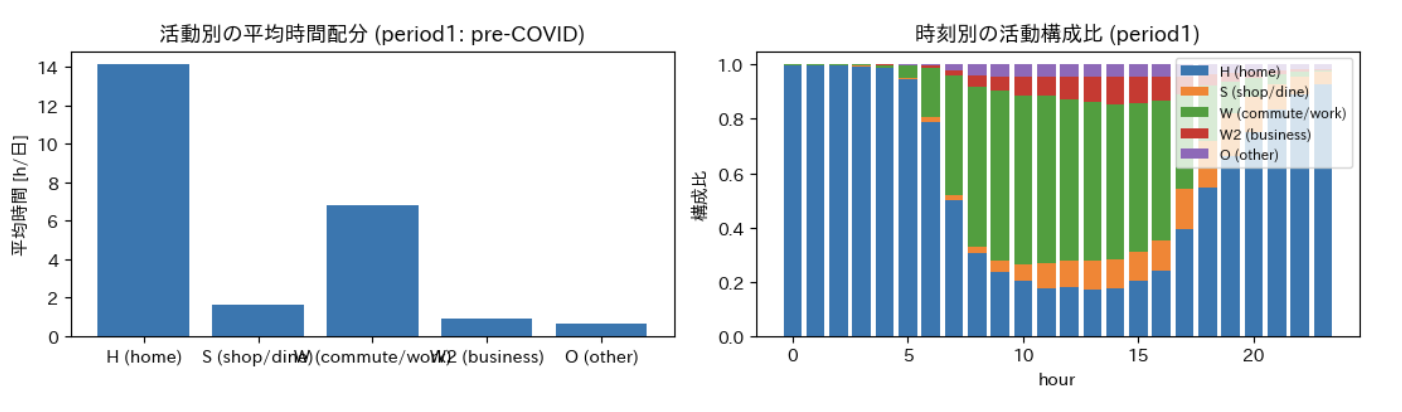
\includegraphics[width=\linewidth]{assets/behavior_modeling/column3/ABMS01.png}
  \captionof{figure}{実データの活動別グラフ}
  \label{fig:activity-graph}
\end{center}

\subsubsection{MDCEVモデル（$\gamma$-profile, Bhat 2008）}

各out活動について，
\begin{equation}
V_k = \psi_k - \log(x_k / \gamma_k + 1)
\end{equation}
ここで，
$\psi_k$：ベース効用，
$x_k$：費やした時間，
$\gamma_k$：飽和パラメータ
である．

選択確率は，以下の閉形式で表される．
\begin{equation}
P(x) = 
\left[ \prod_{k \in M} \frac{1}{x_k + \gamma_k} \right]
\cdot
\left[ \sum_{k \in M} (x_k + \gamma_k) \right]
\cdot
\left[ \prod_{k \in M} \frac{e^{V_k}}{\sum_j e^{V_j}} \right]
\end{equation}

\subsubsection{Recursive Logit Model}

時間$t$における活動，遷移効用を「1時間ごとに次の行動を決める」形で捉えるものとする．
\begin{equation}
U_t(i \to j) =
\alpha_j
+ \delta_{\text{stay}} 1[j = i]
+ \delta_{\text{morn}} 1[i = H, j \neq H, 6 \leq t < 10]
+ \delta_{\text{eve}} 1[i \neq H, j = H, 17 \leq t < 22]
\end{equation}

\subsubsection{分析結果}

\textbf{MDCEVモデル}

\begin{center}
  \renewcommand{\arraystretch}{1.5}
  \setlength{\tabcolsep}{14pt}

  \begin{tabular}{clrrr}
    \toprule
    & \textbf{param} & \textbf{estimate} & \textbf{std\_err} & \textbf{t\_value} \\
    \midrule
    0 & psi\_S           & -0.7392 & 0.0506 & -14.62 \\
    1 & psi\_W           &  0.0295 & 0.0465 &   0.63 \\
    2 & psi\_W2          & -1.7580 & 0.0701 & -25.09 \\
    3 & psi\_O           & -1.9597 & 0.0758 & -25.86 \\
    4 & log\_gamma\_S    &  1.1533 & 0.0736 &  15.67 \\
    5 & log\_gamma\_W    &  2.2314 & 0.0722 &  30.91 \\
    6 & log\_gamma\_W2   &  1.8356 & 0.1202 &  15.27 \\
    7 & log\_gamma\_O    &  1.3246 & 0.1281 &  10.34 \\
    \bottomrule
  \end{tabular}
  \captionof{table}{MDCEVモデル pre コロナ\_MDCEVモデル推定表}
  \label{tab:mdcev-pre-covid}
\end{center}

ベース効用：Hは基準で0であり，ほとんどの活動で0以下なので何もしなければ選ばれにくいことがわかる．

飽和パラメータ：全てプラスの値であり，値が大きいほど，長く続く行動であることがわかる．

$t$値：絶対値が1.96を越えていればそのパラメータは5％有意水準で有意である．

仕事のベース効用が唯一正の値であり大きいので，仕事に行く動機は他の活動と比べて強い．
飽和パラメータが大きいので，仕事は一度始めると比較的長く続くが，買い物，その他は比較的短く切り上げる傾向がある．
仕事の$t$値は低いが，自宅との値の差が小さいためと考えられる．

\textbf{Recursive Logit Model}

\begin{center}
  \renewcommand{\arraystretch}{1.5}
  \setlength{\tabcolsep}{14pt}

  \begin{tabular}{clrrr}
    \toprule
    & \textbf{param} & \textbf{estimate} & \textbf{std\_err} & \textbf{t\_value} \\
    \midrule
    0 & alpha\_S      & -0.2119 & 0.0102 & -20.79 \\
    1 & alpha\_W      & -0.0341 & 0.0062 &  -5.49 \\
    2 & alpha\_W2     & -0.3249 & 0.0141 & -22.97 \\
    3 & alpha\_O      & -0.4137 & 0.0182 & -22.79 \\
    4 & delta\_stay   &  3.6363 & 0.0251 & 145.12 \\
    5 & delta\_morn   &  2.3296 & 0.0608 &  38.35 \\
    6 & delta\_eve    &  2.3148 & 0.0592 &  39.08 \\
    \bottomrule
  \end{tabular}
  \captionof{table}{MDCEVモデルの推定結果}
  \label{tab:mdcev-alpha-delta}
\end{center}

ベース効用：Hが基準で0以下なので何もしなければ選ばれにくい．

活動継続のボーナス：同じ活動を続けることへのボーナスである．

朝の外出ダッシュ：6〜10時の間に自宅を出るボーナスである．

夕方の帰宅ダッシュ：17〜22時の間に自宅に帰るボーナスである．

$\delta_{\text{stay}}$の$t$値が突出して高く，一度始めた活動は継続し続ける傾向があると言える．
また，朝の外出と夕方の帰宅に強いバイアスがあることがわかる．

\textbf{再現性}

モデルから観測時間配分の再現を試みると，RLでは推定パラメータのもとで各user, dayを$t=0$からforward simulateする．
ほとんど完全に表現できていると言える．
朝の外出項などが時間制約の学習に役立っていることがわかる．

\begin{center}
  \renewcommand{\arraystretch}{1.5}
  \setlength{\tabcolsep}{14pt}

  \begin{tabular}{lrr}
    \toprule
    & \textbf{observed [h]} & \textbf{RL simulated [h]} \\
    \midrule
    H (home)            & 14.23 & 14.69 \\
    S (shop/dine)       &  1.65 &  1.67 \\
    W (commute/work)    &  6.61 &  6.13 \\
    W2 (business)       &  0.92 &  0.93 \\
    O (other)           &  0.59 &  0.59 \\
    \bottomrule
  \end{tabular}
  \captionof{table}{RLモデルによる活動時間の再現結果}
  \label{tab:rl-simulated-observed}
\end{center}

\begin{center}
  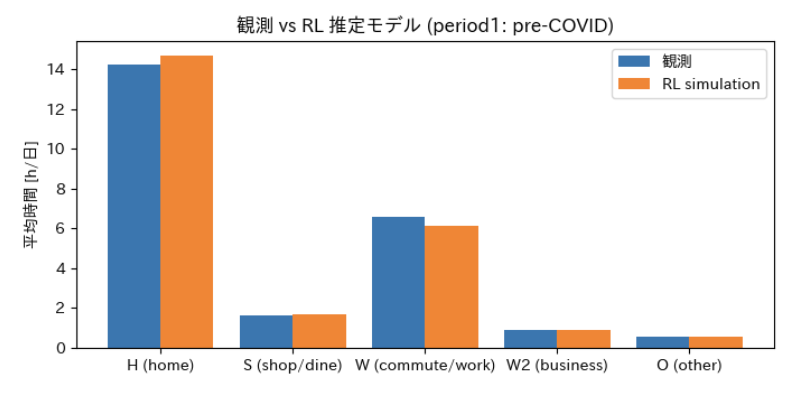
\includegraphics[width=\linewidth]{assets/behavior_modeling/column3/ABMS05-RL.png}
  \captionof{figure}{観測とRLモデルの比較}
  \label{fig:observed-rl-comparison}
\end{center}

\textbf{MDCEVとRLの比較}

両方のモデルから観測時間配分の再現を試す．
MDCEVモデルで推定された$\gamma_k$から求まる期待時間と，RLモデルで推定された$\alpha_k$を比較する．
観測モデルが異なるため直接比較することはできないが，パラメータの符号と各活動の相対的な魅力度の傾向（$\gamma_k$，$\alpha_k$）は一致する．

\begin{center}
  \renewcommand{\arraystretch}{1.3}
  \setlength{\tabcolsep}{6pt}

  \begin{minipage}{0.48\linewidth}
    \centering
    \begin{tabular}{clrrr}
      \toprule
      & \textbf{param} & \textbf{estimate} & \textbf{std\_err} & \textbf{t\_value} \\
      \midrule
      0 & psi\_S           & -0.7392 & 0.0506 & -14.62 \\
      1 & psi\_W           &  0.0295 & 0.0465 &   0.63 \\
      2 & psi\_W2          & -1.7580 & 0.0701 & -25.09 \\
      3 & psi\_O           & -1.9597 & 0.0758 & -25.86 \\
      4 & log\_gamma\_S    &  1.1533 & 0.0736 &  15.67 \\
      5 & log\_gamma\_W    &  2.2314 & 0.0722 &  30.91 \\
      6 & log\_gamma\_W2   &  1.8356 & 0.1202 &  15.27 \\
      7 & log\_gamma\_O    &  1.3246 & 0.1281 &  10.34 \\
      \bottomrule
    \end{tabular}
  \end{minipage}
  \hfill
  \begin{minipage}{0.48\linewidth}
    \centering
    \begin{tabular}{clrrr}
      \toprule
      & \textbf{param} & \textbf{estimate} & \textbf{std\_err} & \textbf{t\_value} \\
      \midrule
      0 & alpha\_S      & -0.2119 & 0.0102 & -20.79 \\
      1 & alpha\_W      & -0.0341 & 0.0062 &  -5.49 \\
      2 & alpha\_W2     & -0.3249 & 0.0141 & -22.97 \\
      3 & alpha\_O      & -0.4137 & 0.0182 & -22.79 \\
      4 & delta\_stay   &  3.6363 & 0.0251 & 145.12 \\
      5 & delta\_morn   &  2.3296 & 0.0608 &  38.35 \\
      6 & delta\_eve    &  2.3148 & 0.0592 &  39.08 \\
      \bottomrule
    \end{tabular}
  \end{minipage}

  \captionof{table}{MDCEVモデルとRLモデルの推定結果の比較}
  \label{tab:mdcev-rl-comparison}
\end{center}

\subsubsection{時期による比較}

\textbf{実データを用いた比較}

・家にいる時間はコロナ規制後，直後ではなく少し経ってから1時間程度長くなっており，仕事・通勤時間は減少した．
コロナ規制後から普及した各種オンラインサービスにより，対面での仕事が減少したのだろうと考えられる．

・Business（業務）は，コロナ規制直後〜翌年の冬にかけて半減していることがわかるが，翌年の秋には元の水準に復活している．

・買い物に使う時間は30分程度増加した．
通勤時間が減り，通勤のついでに買い物に行くということが減って，必要な時間が増えたと考えられる．


\vspace{3pt}

\begin{center}
  \begin{tabular}{lcccc}
    \toprule
    &
    \begin{tabular}[c]{@{}c@{}}Phase1\\ コロナ前\end{tabular}
    &
    \begin{tabular}[c]{@{}c@{}}Phase2\\ コロナ規制直後\end{tabular}
    &
    \begin{tabular}[c]{@{}c@{}}Phase3\\ コロナ後冬\end{tabular}
    &
    \begin{tabular}[c]{@{}c@{}}Phase4\\ コロナ後秋\end{tabular}
    \\
    \midrule
    サンプル数 & 6532 & 2299 & 1394 & 1581 \\
    observed H(home) & 14.23 & 14.77 & 15.49 & 15.45 \\
    observed S(shop/dine) & 1.65 & 1.84 & 1.77 & 2.19 \\
    observed W(commute/work) & 6.61 & 6.54 & 5.56 & 4.73 \\
    observed O(other) & 0.59 & 0.44 & 0.77 & 0.63 \\
    \bottomrule
  \end{tabular}
  \captionof{table}{各Phaseにおける観測活動時間}
  \label{tab:observed-activity-time}
\end{center}

\textbf{RLモデルを用いた比較}

・コロナ規制後，Workの$\alpha$値は下がっている．

・2.コロナ規制直後，3.コロナ後において，ビジネスの$\alpha$値が下がっていることがわかる．
コロナを受けて暫くは出張，訪問が減っていたと言える．

・4.コロナ後秋の結果を見ると，朝の出発に関する$\alpha$値がコロナ前と比べると下がっている．
コロナを経てリモートワークが普及したことにより，朝出勤する人の割合が下がったといえる．

・パラメータで見てもShoppingの$\alpha_k$の値は少し大きくなっている．

\begin{center}
  \renewcommand{\arraystretch}{1.3}
  \setlength{\tabcolsep}{6pt}

  % ===== 1段目 =====
  \begin{minipage}{0.48\linewidth}
    \centering
    \begin{tabular}{clrrr}
      \toprule
      & \textbf{param} & \textbf{estimate} & \textbf{std\_err} & \textbf{t\_value} \\
      \midrule
      0 & alpha\_S    & -0.2119 & 0.0102 & -20.79 \\
      1 & alpha\_W    & -0.0341 & 0.0062 &  -5.49 \\
      2 & alpha\_W2   & -0.3249 & 0.0141 & -22.97 \\
      3 & alpha\_O    & -0.4137 & 0.0182 & -22.79 \\
      4 & delta\_stay &  3.6363 & 0.0251 & 145.12 \\
      5 & delta\_morn &  2.3296 & 0.0608 &  38.35 \\
      6 & delta\_eve  &  2.3148 & 0.0592 &  39.08 \\
      \bottomrule
    \end{tabular}
  \end{minipage}
  \hfill
  \begin{minipage}{0.48\linewidth}
    \centering
    \begin{tabular}{clrrr}
      \toprule
      & \textbf{param} & \textbf{estimate} & \textbf{std\_err} & \textbf{t\_value} \\
      \midrule
      0 & alpha\_S    & -0.2225 & 0.0097 & -22.91 \\
      1 & alpha\_W    & -0.0580 & 0.0061 &  -9.47 \\
      2 & alpha\_W2   & -0.5551 & 0.0237 & -23.42 \\
      3 & alpha\_O    & -0.5360 & 0.0227 & -23.57 \\
      4 & delta\_stay &  3.5142 & 0.0251 & 140.11 \\
      5 & delta\_morn &  2.3911 & 0.0611 &  39.12 \\
      6 & delta\_eve  &  2.0468 & 0.0593 &  34.52 \\
      \bottomrule
    \end{tabular}
  \end{minipage}

  \vspace{1em}

  % ===== 2段目 =====
  \begin{minipage}{0.48\linewidth}
    \centering
    \begin{tabular}{clrrr}
      \toprule
      & \textbf{param} & \textbf{estimate} & \textbf{std\_err} & \textbf{t\_value} \\
      \midrule
      0 & alpha\_S    & -0.2339 & 0.0102 & -22.85 \\
      1 & alpha\_W    & -0.0825 & 0.0066 & -12.46 \\
      2 & alpha\_W2   & -0.5482 & 0.0238 & -23.03 \\
      3 & alpha\_O    & -0.4069 & 0.0167 & -24.29 \\
      4 & delta\_stay &  3.5265 & 0.0257 & 137.35 \\
      5 & delta\_morn &  2.2846 & 0.0630 &  36.25 \\
      6 & delta\_eve  &  2.1253 & 0.0618 &  34.41 \\
      \bottomrule
    \end{tabular}
  \end{minipage}
  \hfill
  \begin{minipage}{0.48\linewidth}
    \centering
    \begin{tabular}{clrrr}
      \toprule
      & \textbf{param} & \textbf{estimate} & \textbf{std\_err} & \textbf{t\_value} \\
      \midrule
      0 & alpha\_S    & -0.1874 & 0.0089 & -21.09 \\
      1 & alpha\_W    & -0.0906 & 0.0067 & -13.59 \\
      2 & alpha\_W2   & -0.3376 & 0.0137 & -24.62 \\
      3 & alpha\_O    & -0.4351 & 0.0179 & -24.24 \\
      4 & delta\_stay &  3.5514 & 0.0240 & 148.00 \\
      5 & delta\_morn &  2.0919 & 0.0598 &  34.99 \\
      6 & delta\_eve  &  2.1750 & 0.0592 &  36.76 \\
      \bottomrule
    \end{tabular}
  \end{minipage}

  \captionof{table}{RLモデルによる時期別推定結果の比較}
  \label{tab:rl-period-comparison}
\end{center}

\textbf{実データとRLモデルの整合性}

・全体的にどの時期のデータについても推定精度は高い．

・4つ全ての時期のデータについて，H在宅を0.5h程度高く見積もる傾向があった．

・4つ全ての時期のデータについて，W通勤・仕事を0.5h程度低く見積もる傾向にあった．

・S買い物，W2業務，Oその他については極めて高い精度で予測できていた．

\begin{center}
  \renewcommand{\arraystretch}{1.4}
  \setlength{\tabcolsep}{10pt}

  % ===== 上段 =====
  \begin{minipage}{0.48\linewidth}
    \centering
    \textbf{時期1}\\[0.3em]
    \begin{tabular}{lrr}
      \toprule
      & \textbf{observed [h]} & \textbf{RL simulated [h]} \\
      \midrule
      H (home)         & 14.23 & 14.69 \\
      S (shop/dine)    &  1.65 &  1.67 \\
      W (commute/work) &  6.61 &  6.13 \\
      W2 (business)    &  0.92 &  0.93 \\
      O (other)        &  0.59 &  0.59 \\
      \bottomrule
    \end{tabular}
  \end{minipage}
  \hfill
  \begin{minipage}{0.48\linewidth}
    \centering
    \textbf{時期2}\\[0.3em]
    \begin{tabular}{lrr}
      \toprule
      & \textbf{observed [h]} & \textbf{RL simulated [h]} \\
      \midrule
      H (home)         & 14.77 & 15.25 \\
      S (shop/dine)    &  1.84 &  1.83 \\
      W (commute/work) &  6.54 &  6.10 \\
      W2 (business)    &  0.42 &  0.38 \\
      O (other)        &  0.44 &  0.44 \\
      \bottomrule
    \end{tabular}
  \end{minipage}

  \vspace{1em}

  % ===== 下段 =====
  \begin{minipage}{0.48\linewidth}
    \centering
    \textbf{時期3}\\[0.3em]
    \begin{tabular}{lrr}
      \toprule
      & \textbf{observed [h]} & \textbf{RL simulated [h]} \\
      \midrule
      H (home)         & 15.49 & 15.88 \\
      S (shop/dine)    &  1.77 &  1.78 \\
      W (commute/work) &  5.56 &  5.19 \\
      W2 (business)    &  0.43 &  0.41 \\
      O (other)        &  0.74 &  0.74 \\
      \bottomrule
    \end{tabular}
  \end{minipage}
  \hfill
  \begin{minipage}{0.48\linewidth}
    \centering
    \textbf{時期4}\\[0.3em]
    \begin{tabular}{lrr}
      \toprule
      & \textbf{observed [h]} & \textbf{RL simulated [h]} \\
      \midrule
      H (home)         & 15.45 & 15.84 \\
      S (shop/dine)    &  2.19 &  2.26 \\
      W (commute/work) &  4.73 &  4.29 \\
      W2 (business)    &  0.99 &  1.00 \\
      O (other)        &  0.63 &  0.60 \\
      \bottomrule
    \end{tabular}
  \end{minipage}

  \captionof{table}{RLモデルによる時期別活動時間の比較}
  \label{tab:rl-time-comparison-periods}
\end{center}

\subsubsection{MDCEVモデルのforecast}

Bhat(2008)のForecasting Algorithm（決定論的最適配分）を用いる．

・MDCEVモデルではW(通勤，仕事)を多く見積もる傾向がある．

・RLモデルの方がS，W2，Oの活動時間を正確に見積もることができている．

\begin{center}
  \renewcommand{\arraystretch}{1.5}
  \setlength{\tabcolsep}{14pt}

  \begin{tabular}{lrrr}
    \toprule
    & \textbf{observed [h]} & \textbf{MDCEV pred (obs active set) [h]} & \textbf{diff} \\
    \midrule
    H  & 14.229 & -0.000 & -14.229 \\
    S  &  1.648 &  1.440 &  -0.208 \\
    W  &  6.615 &  7.621 &   1.007 \\
    W2 &  0.918 &  0.337 &  -0.581 \\
    O  &  0.590 &  0.372 &  -0.218 \\
    \bottomrule
  \end{tabular}
  \captionof{table}{MDCEVモデルによる活動時間の予測結果}
  \label{tab:mdcev-pred-obs-active-set}
\end{center}

\begin{center}
  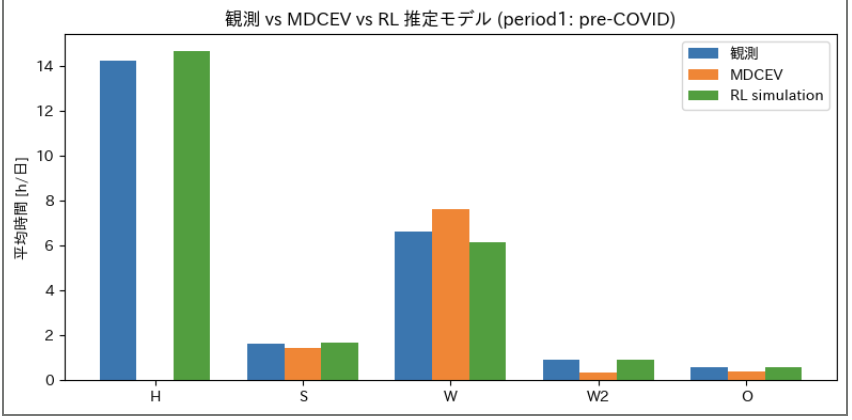
\includegraphics[width=\linewidth]{assets/behavior_modeling/column3/ABMS10.png}
  \captionof{figure}{実データとRLデータの整合性}
  \label{fig:observed-rl-consistency-2}
\end{center}

\subsubsection{Day-to-Day Dynamics}

通常のRecursive Logit Modelでは，過去の活動履歴を考慮することはできないが，ここに
\textbf{全ての活動に対して同じパラメータを追加する場合}を考える．
1日の各活動の最後に行った日からの経過日数も考慮に入れる．

\begin{equation}
U_t(i \to j) = [\text{baseline}] + \theta_{\text{rec}} \cdot \text{recency}_u(a(j))
\end{equation}

\begin{center}
  \renewcommand{\arraystretch}{1.5}
  \setlength{\tabcolsep}{14pt}

  \begin{tabular}{clrrr}
    \toprule
    & \textbf{param} & \textbf{estimate} & \textbf{std\_err} & \textbf{t\_value} \\
    \midrule
    0 & alpha\_S        & -0.1449 & 0.0109 & -13.27 \\
    1 & alpha\_W        &  0.0065 & 0.0068 &   0.96 \\
    2 & alpha\_W2       & -0.2210 & 0.0156 & -14.13 \\
    3 & alpha\_O        & -0.3076 & 0.0194 & -15.89 \\
    4 & delta\_stay     &  3.6110 & 0.0251 & 144.14 \\
    5 & delta\_morn     &  2.3335 & 0.0606 &  38.52 \\
    6 & delta\_eve      &  2.3115 & 0.0592 &  39.04 \\
    7 & theta\_recency  & -0.0387 & 0.0028 & -13.84 \\
    \bottomrule
  \end{tabular}
  \captionof{table}{Day-to-Day Dynamics}
  \label{tab:day-to-day-dynamics}
\end{center}

$\theta_{\text{rec}} < 0$より，普段やらない活動は将来も選ばれにくい傾向にあるといえる．
recencyを入れた方が，Wの時間については正確に推定することができていた．

\begin{center}
  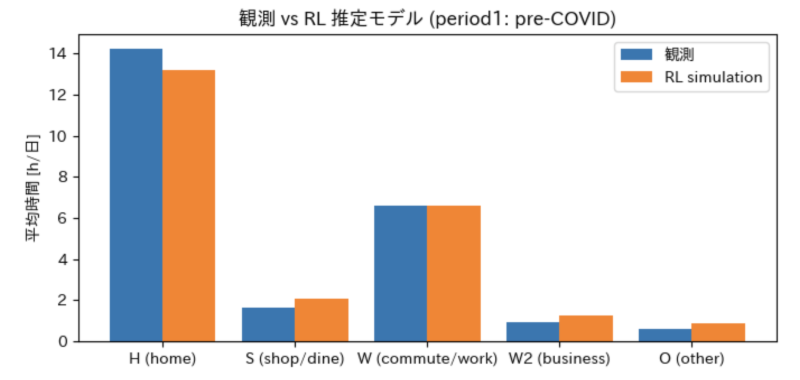
\includegraphics[width=\linewidth]{assets/behavior_modeling/column3/ABMS12.png}
  \captionof{figure}{キャプション}
  \label{fig:recency-result}
\end{center}

\textbf{活動種類ごとのDay-to-Day Recencyを導入する場合}

活動ごとの個別のパラメータの導入を行い，各活動ごとに違いを見た．
レコードごとに効用が異なるので，$N$個の異なる効用関数を解くことで，一人一人の現在の状況に合わせた将来予測を計算する．

\begin{center}
  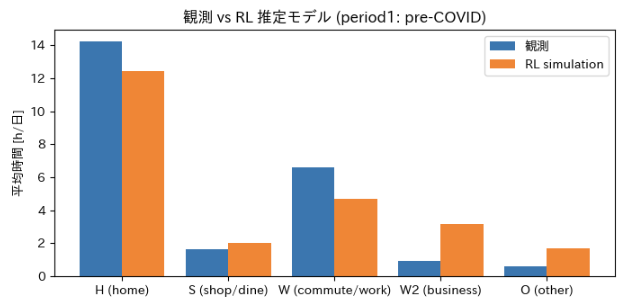
\includegraphics[width=\linewidth]{assets/behavior_modeling/column3/ABMS13.png}
  \captionof{figure}{キャプション}
  \label{fig:activity-specific-recency}
\end{center}

モデルのはまり具合は悪化してしまったが，これはW2(Business)は他の活動と比べて発生頻度が低いため，負の相関を強く見積り過ぎた結果，シミュレーション上ではW2が過剰に選ばれる事態が発生してしまったのではないかと考えられる．
さらに，サンプル数が少ないため，個人の極端な行動の影響を受けている可能性が高い．

\end{column}
\clearpage